
%%%%%%%%%%%%%%%%%%%%%%%%%%%%%%%%%%%%%%%%%%%%%%%%%%%%%%%%%%%%%
\subsubsection{模型建立}

针对问题二，本节将从工况划分、约束优化模型建立和求解策略三个角度展开。具体过程如下。

\textbf{步骤1：K-Means工况划分}

将$(C_{in},T_{in},Q)$三维标准化空间划分为$K$个典型工况$\Omega_k$，满足：
\begin{equation}
    \bigcup_{k=1}^{K} \Omega_k = \Omega_{all},\quad \Omega_j \cap \Omega_k = \emptyset\;(j\neq k)
\end{equation}

轮廓系数定义为：
\begin{equation}
    s_i = \frac{b_i - a_i}{\max(a_i, b_i)}
\end{equation}
其中$a_i$为样本到同簇其他点平均距离，$b_i$为到最近异簇平均距离，$s_i\in[-1,1]$越大表示聚类越紧凑分离。在$K\in[2,8]$范围内选取轮廓系数最大且每工况样本占比$\geq 3\%$的$K$值。

\textbf{步骤2：约束优化模型}

每个工况下决策变量为$[U_1,U_2,U_3,U_4,T_1,T_2,T_3,T_4]$共8维，优化模型为：
\begin{equation}
    \min_{U_i,T_i}\ P_{total} = \sum_{i=1}^{4} k_i U_i^2 + \sum_{i=1}^{4} \frac{\beta_i}{T_i} + c
\end{equation}
\begin{equation}
    \text{s.t.}\quad C_{out}(T_{in}^{(k)},C_{in}^{(k)},Q^{(k)},U,T) \leq C_{limit}
\end{equation}
\begin{equation}
    U_{min,i} \leq U_i \leq U_{max,i},\quad i=1,2,3,4
\end{equation}
\begin{equation}
    T_{min,i} \leq T_i \leq \min(T_{max,i},\,T_{crit,i}),\quad i=1,2,3,4
\end{equation}

目标函数同时含电压和振打，振打通过$\beta_i/T_i$项直接参与目标优化，同时也通过约束（影响$C_{out}$）间接参与。

\textbf{步骤3：求解策略}

采用SLSQP（Sequential Least SQuares Programming）算法\cite{nocedal2006}求解，该算法属于序列二次规划类，在约束边界附近用二次近似，对中等规模（8维）带不等式约束的非线性优化效果好。因约束$C_{out}\leq 10$在8维空间定义的可行域可能非凸，单起点易陷局部最优，故采用多起点策略（10个起点）：第0个起点取边界中点，其余9个在边界内随机均匀采样，取目标最小且满足约束的解。固定随机种子42保证可复现。

当SLSQP全部起点不收敛或约束不满足时，切换差分进化全局备选算法，将约束罚入目标：
\begin{equation}
    \tilde{P}(x) = \begin{cases} P_{total}(x), & C_{out} \leq C_{limit} \\ 10^6 + (C_{out} - C_{limit})\times 10^4, & C_{out} > C_{limit} \end{cases}
\end{equation}

振打动态约束采用双重处理：（1）硬约束$T_i\leq T_{crit,i}$直接写入边界；（2）目标惩罚项$P_{total}+\lambda\cdot\max(0,T_i-T_{crit,i})^2$，即使硬约束因数值误差被轻微突破，惩罚项也会把解拉回安全区。

% ============================================================
\subsubsection{模型求解}

基于上述模型，对6个典型工况分别求解约束优化问题，结果如表\ref{tab:问题2结果}所示。

\begin{table}[H]
  \centering
  \caption{问题二各工况最优操作参数与电耗}
  \label{tab:问题2结果}
  \zihao{-5}
  \renewcommand{\arraystretch}{1.1}
  \begin{tabular}{ccccccccccccc}
    \toprule
    工况 & 样本数 & $C_{in}$ & $T_{in}$ & $U_1$ & $U_2$ & $U_3$ & $U_4$ & $T_1$ & $T_2$ & $T_3$ & $T_4$ & $P^*$(kW) \\
    \midrule
    0 & 1309 & 44.34 & 119.5 & 85.1 & 66.3 & 38.0 & 37.0 & 233 & 233 & 472 & 472 & 1992.8 \\
    1 & 2184 & 26.60 & 131.4 & 85.1 & 50.0 & 38.0 & 37.0 & 233 & 233 & 472 & 472 & 1831.4 \\
    2 & 1009 & 43.77 & 131.4 & 85.1 & 57.0 & 38.0 & 37.0 & 233 & 233 & 472 & 472 & 1894.9 \\
    3 & 1583 & 42.93 & 119.9 & 85.1 & 56.5 & 38.0 & 37.0 & 233 & 233 & 472 & 472 & 1890.3 \\
    4 & 2360 & 40.19 & 130.0 & 85.1 & 65.3 & 38.0 & 37.0 & 233 & 233 & 472 & 472 & 1981.1 \\
    5 & 1635 & 26.01 & 120.8 & 85.1 & 58.7 & 38.0 & 37.0 & 233 & 233 & 472 & 472 & 1911.8 \\
    \bottomrule
  \end{tabular}
\end{table}

各工况最优解均满足$C_{out}=10.0\;\text{mg/Nm}^3$的排放约束。K-Means工况划分结果如图\ref{fig:regime_scatter}所示，6个工况在$(C_{in},T_{in})$空间中分布合理，区间内相近、区间间差异明显。

\begin{figure}[H]
  \centering
  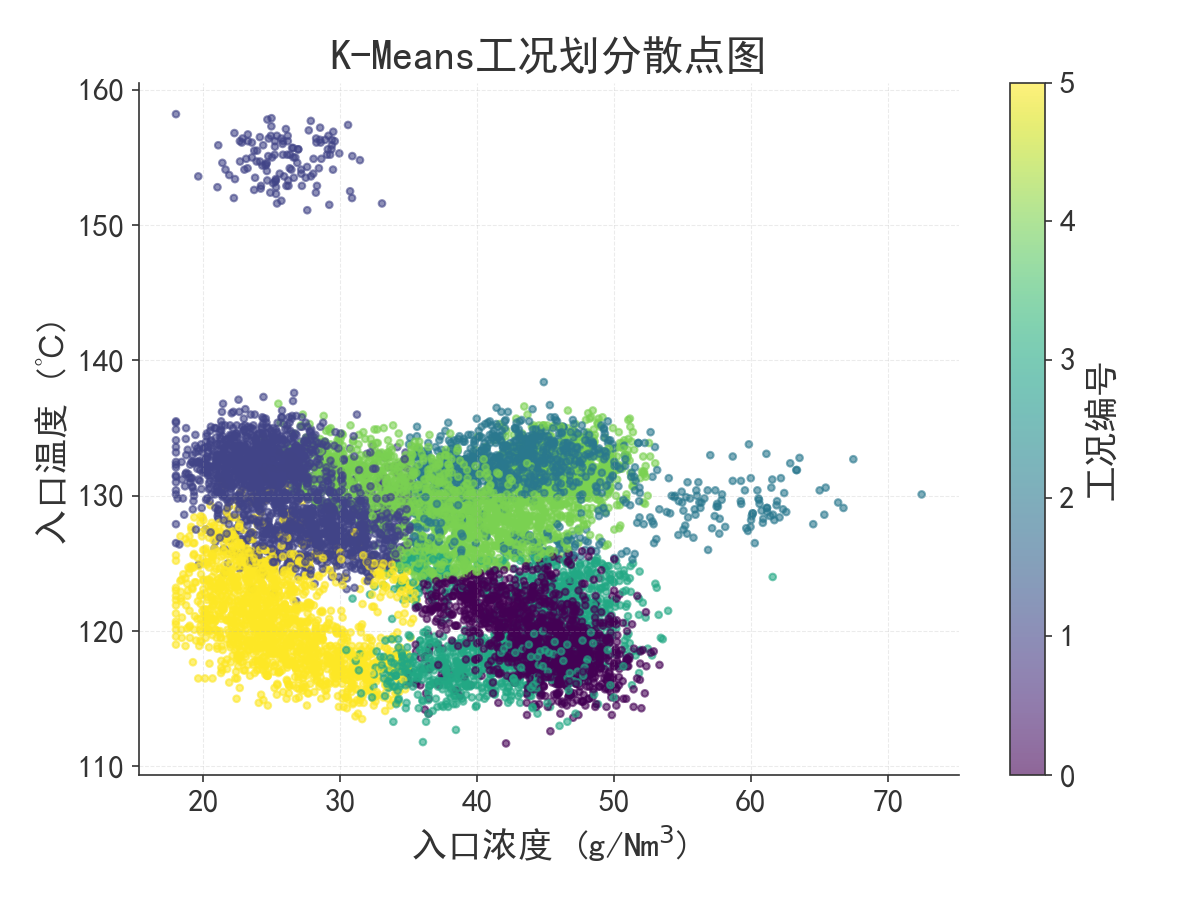
\includegraphics[width=0.75\textwidth]{figures/regime_scatter.png}
  \caption{K-Means工况划分散点图}
  \label{fig:regime_scatter}
\end{figure}

分析结果可见：

（1）高浓度工况（工况0，$C_{in}=44.34$）最优电耗$P^*=1992.8\;\text{kW}$最高，低浓度工况（工况1，$C_{in}=26.60$）$P^*=1831.4\;\text{kW}$最低，电耗随入口浓度递增，符合物理规律。

（2）各工况$U_1$均贴上界85.1\,kV，$U_3$均贴下界38.0\,kV，$U_4$均贴下界37.0\,kV，说明第1电场电压对降低$C_{out}$贡献最大；$U_2$在内部调节，是各工况差异化调节的主要自由度。

（3）各工况振打周期均取历史中位数（$T_1=T_2=233$\,s，$T_3=T_4=472$\,s），因双向偏离模型使$T_{ref,i}$处效率最高，优化器自然选择参考值附近，避免过频或过疏振打。

\textbf{振打同步性分析。}对历史数据计算同电场组振打周期比值，前两电场$T_1/T_2$均值$=1.003$，后两电场$T_3/T_4$均值$=1.001$，表明数据中前两电场和后两电场各自同步振打。同步振打虽便于控制，但多电场同时振打瞬间脱落粉尘叠加，瞬时排放峰值显著增大。错峰策略（如$T_1$与$T_2$错开半周期）可降低峰值$C_{peak}$，初步估算错峰后峰值可降至同步模式的约$1/\sqrt{2}$，值得在工程中优先采用。
